% Generated by code/needham.py -- do not edit by hand.
\definecolor{qocA}{rgb}{0.00,0.45,0.70}
\definecolor{qocB}{rgb}{0.90,0.60,0.00}
\definecolor{qocC}{rgb}{0.00,0.62,0.45}
\definecolor{qocD}{rgb}{0.80,0.40,0.00}
\definecolor{qocE}{rgb}{0.80,0.60,0.70}
\definecolor{qocF}{rgb}{0.35,0.70,0.90}
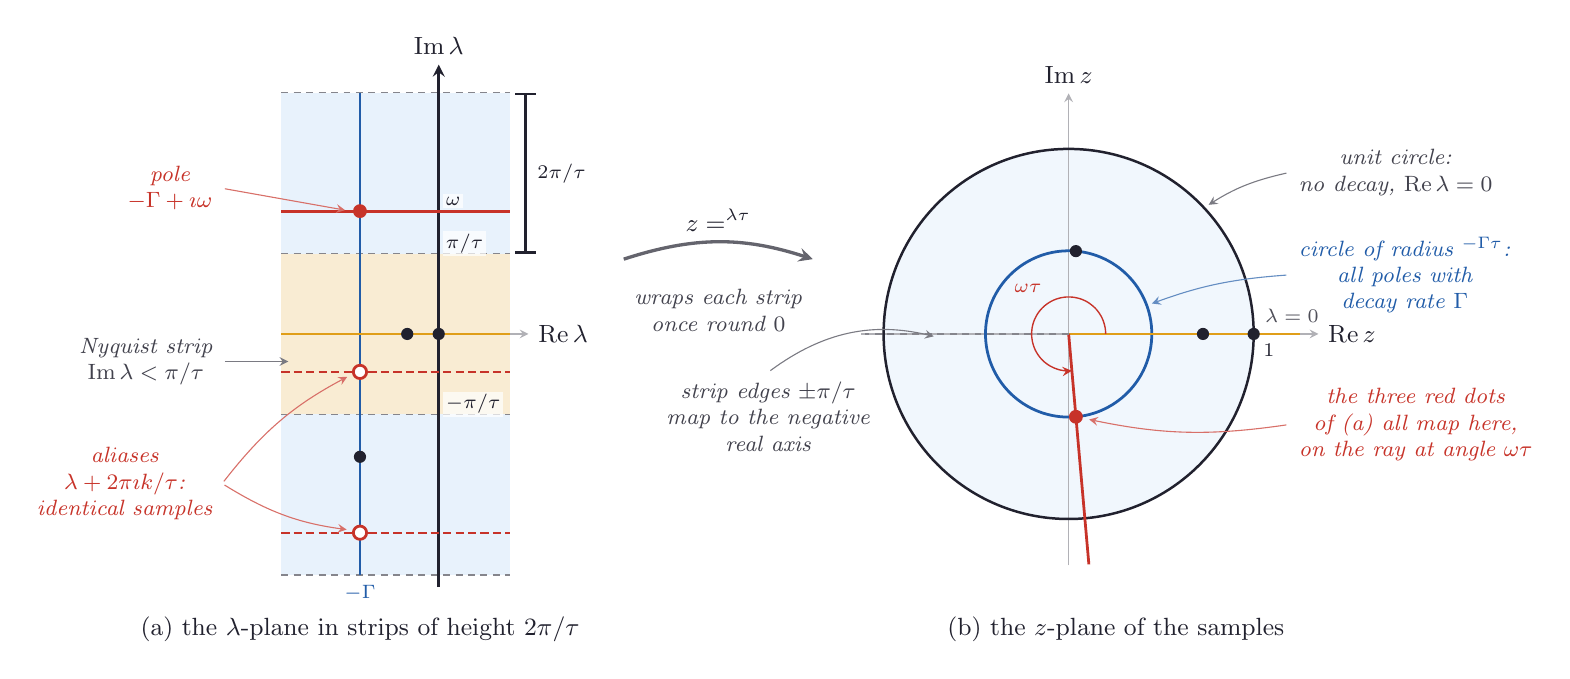
\begin{tikzpicture}[ink/.style={line width=0.9pt, ndInk}, faint/.style={line width=0.4pt, ndInk!35}, dashedink/.style={line width=0.5pt, ndInk!55, dash pattern=on 2.5pt off 2pt}, vec/.style={->, >=stealth, line width=1.2pt}, note/.style={font=\footnotesize\itshape, text=ndInk!85, align=center}, pointer/.style={->, >=stealth, line width=0.4pt, ndInk!60, shorten >=2pt, shorten <=1pt}, dot/.style={circle, fill=ndInk, inner sep=0pt, minimum size=3.4pt}, wash/.style={fill=ndSky, fill opacity=0.55}, every node/.style={text=ndInk}]
\definecolor{ndInk}{rgb}{0.13,0.13,0.18}
\definecolor{ndPaper}{rgb}{0.99,0.96,0.88}
\definecolor{ndSky}{rgb}{0.84,0.91,0.98}
\definecolor{ndRose}{rgb}{0.98,0.86,0.84}
\definecolor{ndBlue}{rgb}{0.13,0.36,0.66}
\definecolor{ndRed}{rgb}{0.78,0.20,0.16}
\definecolor{ndGold}{rgb}{0.88,0.62,0.10}
\definecolor{ndGreen}{rgb}{0.18,0.52,0.30}
\fill[ndSky, fill opacity=0.55] (1.000,-3.063) rectangle (3.900,-1.021);
\fill[ndGold!35, fill opacity=0.55] (1.000,-1.021) rectangle (3.900,1.021);
\fill[ndSky, fill opacity=0.55] (1.000,1.021) rectangle (3.900,3.063);
\draw[dashedink] (1.000,-3.063) -- (3.900,-3.063);
\draw[dashedink] (1.000,-1.021) -- (3.900,-1.021);
\draw[dashedink] (1.000,1.021) -- (3.900,1.021);
\draw[dashedink] (1.000,3.063) -- (3.900,3.063);
\draw[faint, ->, >=stealth] (1.000,0.000) -- (4.140,0.000) node[right, text=ndInk, font=\small] {$\mathrm{Re}\,\lambda$};
\draw[ink, ->, >=stealth] (3.000,-3.216) -- (3.000,3.420) node[above, text=ndInk, font=\small] {$\mathrm{Im}\,\lambda$};
\draw[line width=1.0pt, ndBlue] (2.000,-3.063) -- (2.000,3.063);
\draw[line width=0.6pt, dash pattern=on 3pt off 1.5pt, ndRed] (1.000,-2.524) -- (3.900,-2.524);
\draw[line width=0.6pt, dash pattern=on 3pt off 1.5pt, ndRed] (1.000,-0.482) -- (3.900,-0.482);
\draw[line width=1.0pt, ndRed] (1.000,1.560) -- (3.900,1.560);
\draw[line width=1.0pt, ndGold] (1.000,0.000) -- (3.900,0.000);
\node[font=\scriptsize, anchor=west, fill=white, fill opacity=0.7, text opacity=1, inner sep=1pt] at (3.050,1.151) {$\pi/\tau$};
\node[font=\scriptsize, anchor=west, fill=white, fill opacity=0.7, text opacity=1, inner sep=1pt] at (3.050,-0.891) {$-\pi/\tau$};
\node[font=\scriptsize, anchor=west, fill=white, fill opacity=0.7, text opacity=1, inner sep=1pt] at (3.050,1.690) {$\omega$};
\node[font=\scriptsize, text=ndBlue, below] at (2.000,-3.063) {$-\Gamma$};
\draw[ink, |-|] (4.100,1.021) -- (4.100,3.063);
\node[font=\scriptsize, anchor=west] at (4.130,2.042) {$2\pi/\tau$};
\node[dot, minimum size=4.4pt] at (3.000,0.000) {};
\node[dot, minimum size=4.4pt] at (2.600,0.000) {};
\node[dot, minimum size=4.4pt] at (2.000,-1.560) {};
\draw[ndRed, line width=1pt, fill=white] (2.000,-2.524) circle (2.4pt);
\draw[ndRed, line width=1pt, fill=white] (2.000,-0.482) circle (2.4pt);
\node[dot, fill=ndRed, minimum size=5pt] at (2.000,1.560) {};
\node[note, anchor=east] (ny) at (0.250,-0.350) {Nyquist strip\\ $\abs{\mathrm{Im}\,\lambda}<\pi/\tau$};
\draw[pointer] (ny.east) -- (1.160,-0.350);
\node[note, anchor=east, text=ndRed] (al) at (0.250,-1.900) {aliases\\ $\lambda+2\pi\imath k/\tau$:\\ identical samples};
\draw[pointer, ndRed!70] (al.east) to[bend right=12] (1.900,-2.494);
\draw[pointer, ndRed!70] (al.east) to[bend left=12] (1.900,-0.512);
\node[note, anchor=east, text=ndRed] (pl) at (0.250,1.850) {pole\\ $-\Gamma+\imath\omega$};
\draw[pointer, ndRed!70] (pl.east) -- (1.880,1.560);
\draw[vec, ndInk!70] (5.35,0.95) to[bend left=18] node[above, font=\small, text=ndInk] {$z=\ee^{\lambda\tau}$} (7.75,0.95);
\node[note] at (6.55,0.3) {wraps each strip\\ once round $0$};
\fill[ndSky, fill opacity=0.35] (11.000,0.000) circle (2.350);
\draw[faint, ->, >=stealth] (8.368,0.000) -- (14.172,0.000) node[right, text=ndInk, font=\small] {$\mathrm{Re}\,z$};
\draw[faint, ->, >=stealth] (11.000,-2.938) -- (11.000,3.055) node[above, text=ndInk, font=\small] {$\mathrm{Im}\,z$};
\draw[ink] (11.000,0.000) circle (2.350);
\draw[line width=1.0pt, ndBlue] (11.000,0.000) circle (1.056);
\draw[line width=1.0pt, ndGold] (11.000,0.000) -- (13.938,0.000);
\draw[line width=1.0pt, ndRed] (11.000,0.000) -- (11.257,-2.926);
\draw[dashedink, line width=0.8pt] (11.000,0.000) -- (8.415,0.000);
\draw[line width=0.5pt, ndRed, ->, >=stealth] (11.470,0.000) -- (11.469,0.029) -- (11.467,0.057) -- (11.462,0.085) -- (11.456,0.113) -- (11.448,0.141) -- (11.439,0.168) -- (11.428,0.194) -- (11.416,0.220) -- (11.401,0.244) -- (11.386,0.268) -- (11.369,0.291) -- (11.351,0.313) -- (11.331,0.334) -- (11.310,0.353) -- (11.288,0.371) -- (11.265,0.388) -- (11.241,0.404) -- (11.216,0.418) -- (11.190,0.430) -- (11.164,0.441) -- (11.137,0.450) -- (11.109,0.457) -- (11.081,0.463) -- (11.053,0.467) -- (11.024,0.469) -- (10.996,0.470) -- (10.967,0.469) -- (10.939,0.466) -- (10.911,0.461) -- (10.883,0.455) -- (10.855,0.447) -- (10.829,0.438) -- (10.802,0.426) -- (10.777,0.414) -- (10.752,0.399) -- (10.728,0.383) -- (10.705,0.366) -- (10.684,0.348) -- (10.663,0.328) -- (10.644,0.307) -- (10.626,0.285) -- (10.609,0.261) -- (10.594,0.237) -- (10.581,0.212) -- (10.568,0.186) -- (10.558,0.160) -- (10.549,0.133) -- (10.542,0.105) -- (10.536,0.077) -- (10.533,0.049) -- (10.530,0.020) -- (10.530,-0.008) -- (10.531,-0.037) -- (10.535,-0.065) -- (10.539,-0.093) -- (10.546,-0.121) -- (10.554,-0.149) -- (10.564,-0.175) -- (10.575,-0.202) -- (10.588,-0.227) -- (10.603,-0.252) -- (10.619,-0.275) -- (10.636,-0.298) -- (10.655,-0.319) -- (10.675,-0.340) -- (10.696,-0.359) -- (10.719,-0.377) -- (10.742,-0.393) -- (10.766,-0.408) -- (10.792,-0.421) -- (10.818,-0.433) -- (10.844,-0.443) -- (10.871,-0.452) -- (10.899,-0.459) -- (10.927,-0.464) -- (10.956,-0.468) -- (10.984,-0.470) -- (11.013,-0.470) -- (11.041,-0.468);
\node[font=\scriptsize, text=ndRed] at (10.483,0.578) {$\omega\tau$};
\node[dot, minimum size=4.4pt] at (13.350,0.000) {};
\node[dot, minimum size=4.4pt] at (12.706,0.000) {};
\node[dot, fill=ndRed, minimum size=5pt] at (11.092,-1.052) {};
\node[dot, minimum size=4.4pt] at (11.092,1.052) {};
\node[note, anchor=west] (uc) at (13.800,2.050) {unit circle:\\ no decay, $\mathrm{Re}\,\lambda=0$};
\draw[pointer] (uc.west) to[bend right=10] (12.719,1.602);
\node[note, anchor=west, text=ndBlue] (bc) at (13.800,0.750) {circle of radius $\ee^{-\Gamma\tau}$:\\ all poles with\\ decay rate $\Gamma$};
\draw[pointer, ndBlue!70] (bc.west) to[bend right=8] (11.992,0.362);
\node[note, anchor=west, text=ndRed] (rz) at (13.800,-1.150) {the three red dots\\ of (a) all map here,\\ on the ray at angle $\omega\tau$};
\draw[pointer, ndRed!70] (rz.west) to[bend left=10] (11.192,-1.072);
\node[note, anchor=east] (ng) at (8.600,-1.050) {strip edges $\pm\pi/\tau$\\ map to the negative\\ real axis};
\draw[pointer] (ng.north) to[bend left=25] (9.355,-0.047);
\node[font=\scriptsize, anchor=north west] at (13.350,0.000) {$1$};
\node[font=\scriptsize, text=ndInk!80, anchor=south west] at (13.370,0.020) {$\lambda=0$};
\node[font=\small] at (2.000,-3.750) {(a) the $\lambda$-plane in strips of height $2\pi/\tau$};
\node[font=\small] at (11.600,-3.750) {(b) the $z$-plane of the samples};
\end{tikzpicture}
